\documentclass{article}


\usepackage{arxiv}

\usepackage[utf8]{inputenc} % allow utf-8 input
\usepackage[T1]{fontenc}    % use 8-bit T1 fonts
\usepackage{hyperref}       % hyperlinks
\usepackage{url}            % simple URL typesetting
\usepackage{booktabs}       % professional-quality tables
\usepackage{amsfonts}       % blackboard math symbols
\usepackage{nicefrac}       % compact symbols for 1/2, etc.
\usepackage{microtype}      % microtypography
\usepackage{lipsum}
\usepackage{listings}
\usepackage{color}
\usepackage{graphicx}

\definecolor{dkgreen}{rgb}{0,0.6,0}
\definecolor{gray}{rgb}{0.5,0.5,0.5}
\definecolor{mauve}{rgb}{0.58,0,0.82}

\title{Evolution to Find Evolution}


\lstset{frame=tb,
  language=PHP,
  aboveskip=3mm,
  belowskip=3mm,
  showstringspaces=false,
  columns=flexible,
  basicstyle={\small\ttfamily},
  numbers=none,
  numberstyle=\tiny\color{gray},
  keywordstyle=\color{blue},
  commentstyle=\color{dkgreen},
  stringstyle=\color{mauve},
  breaklines=true,
  breakatwhitespace=true,
  tabsize=3
}


\author{
  Amelia Berle\\%\thanks{Use footnote for providing further
    %information about author (webpage, alternative
    %address)---\emph{not} for acknowledging funding agencies.} \\
   Biology \& Computer Science Major\\
  Lewis \& Clark College\\
  Portland, OR 97219 \\
  \texttt{ameliaberle@lclark.edu} \\
  %% examples of more authors
   %\And
 %Elias D.~Striatum \\
  %Department of Electrical Engineering\\
  %Mount-Sheikh University\\
  %Santa Narimana, Levand \\
  %\texttt{stariate@ee.mount-sheikh.edu} \\
  %% \AND
  %% Coauthor \\
  %% Affiliation \\
  %% Address \\a
  %% \texttt{email} \\
  %% \And
  %% Coauthor \\
  %% Affiliation \\
  %% Address \\
  %% \texttt{email} \\
  %% \And
  %% Coauthor \\
  %% Affiliation \\
  %% Address \\
  %% \texttt{email} \\
}

\begin{document}
\maketitle

\begin{abstract}
As genetic sequencing becomes faster, more accurate, and more efficient, enormous new datasets are being gathered, but the processing and interpreting of the data has not seen quite as large of an improvement.  dN/dS ratios can be used as an approximate measure to determine if a genetic sequence is undergoing selection and in which direction.  In this project, we explore using genetic algorithms and dN/dS ratios to find areas in a sequence which are experiencing selection.  Preliminary results indicate that this approach could be useful for highlighting areas in which selection is occurring.
\end{abstract}


% keywords can be removed
\keywords{Bioinformatics \and Genetic Algorithms \and dN/dS \and Evolution \and Python \and DNA Analysis \and Mutations
}


\section{Introduction}
	Currently there is a wealth of information available through genetic sequencing.  There are many freely available, large datasets of genetic sequences online and they are growing rapidly.  Much effort is being expended to analyze this data, but because the data can be used for many different analyses there still remains a lot of work to do[1,2].  This project was started with the goal of creating a tool to help find areas of interest in DNA sequences so that those areas can be analyzed.
Proteins are made out of amino acids, each amino acid is coded for with a triplet of DNA nucleotides called a codon.  Multiple codons can code for the same amino acid[3].  A synonymous mutation is one where the change in the DNA sequence does not change the amino acid sequence that is created.  A nonsynonymous mutation is one which changes the amino acid that is coded for[2,4].  dN/dS, the ratio of nonsynonymous mutations to nonsynonymous sites over the ratio of synonymous mutations to synonymous sites, (Equation 1), is a measure of selection[2,5].  Because selective pressures on synonymous mutations are so small and the likelihood of mutation is similar for each site, the ratio of synonymous mutations to synonymous sites is used as an estimate of the mutation rate.  The ratio of nonsynonymous mutations to nonsynonymous sites would be roughly equal to the base mutation rate if the area was experiencing no selection.  This would mean a dN/dS value of ~1.  If the value is greater than one, then the area is experiencing selection in favor of mutations.  Likewise, if the value is less than one, then the area is experiencing purifying selection [2]. This equation assumes that the frequency of synonymous mutations reflects the mutation rate. It also assumes that selection on synonymous sites is negligible. Additionally, it is only useful when applied to related sequences.  If it is run on an alignment where the sequences are unrelated then it cannot give any information on selective pressures. 
        	Genetic algorithms are intended to mimic evolution.  Different ‘genes’, individual bits, are turned on and off.  These make up part of a string of bits known as an ‘individual’ or a ‘chromosome.’  The collection of individuals is called a population. The ones that score the best with a fitness function are crossed and used to make the next ‘generation.’  This process continues and the result is a string of bits which were the most successful at the fitness function[6].  If the fitness function is designed well, then the string of bits should be a good answer to the question.

\section{Methods}
Python was the language chosen for this project because of the many bioinformatics packages available for it.  Biopython[7] was the package chosen for converting between filetypes and Pyevolve[8] was used for genetic algorithm creation. The program reads in an alignment file and then traverses it codon by codon determining whether or not a mutation happened there and if it is synonymous or not.  During this process it creates a string indicating whether or not that codon has a mutation and if the middle site is synonymous or nonsynonymous.  The fitness function goes through each group of turned on bits, if the group is too small it subtracts a penalty from the fitness score. For every zero it adds a bonus because otherwise the algorithm would favor having every bit turned on.  After that, it adds to the fitness based on the dN/dS score of the group.  The score is then divided by the number of groups and returned as the fitness.  The original design of the program was to differentiate between selection for and against change, but that requires further work.

\section{Results}
The output of this program has returned the kind of results we were aiming for (Figure 1), alternating groups of ‘on’ and ‘off’ where the ‘on’ bits correspond to the areas in which mutations are, but still frequently does not.  When the fitness function is adjusted to use different values, the number of bits in the places we expect them moves up or down in relation.  The best scores so far have been obtained by having a punishment of -3 for a group that is too small and a benefit of 0.5 for each zero in the individual (Figure 2).

\section{Discussion}
The results show potential, but the program needs further fine-tuning before it can be applied with practical results.  There are a number of things which can be adjusted to improve its usefulness and accuracy, but unfortunately those were beyond the time constraints of this project.  Given more time, the project would have benefited by edits to take in larger alignment files.  Additionally, the program has not been tested on natural DNA sequences, instead it has only been run on test sequences.  The current version cannot handle gaps in the sequence and because gaps are fairly common in alignments this severely limits the sequences the program can be run on. The fitness function still needs some work on balancing it and we have not yet explored how changes in the mutation rate or crossover type will change this program.  While the program is being improved, it still needs more work before it can be put to practical use.
Despite the fact that the program still needs calibration, the concept behind it seems to be working. When the values of the fitness function are not too far askew, the average fitness of each generation trends upward as the program runs.  The program has given output following the general pattern we are aiming for, a series of ‘on’ groups roughly matching the areas of mutations, and has shown improvement in scores when the fitness function is adjusted.

\begin{figure}
    \centering
    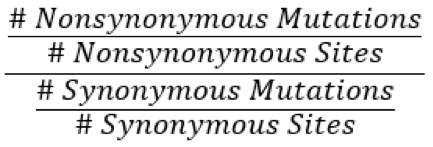
\includegraphics{amelia_fig1.png}
    \caption{\textbf{The dN/dS calculation.}  It is the ratio of nonsynonymous mutations to nonsynonymous sites over the ratio of synonymous mutations to synonymous sites.  dN/dS is used as a measure of selection with values near one indicating no selection, values greater than one indicating selection in favor of the mutations, and values less than one indicating selection against change}
    \label{fig:my_label}
\end{figure}

\begin{figure}
    \centering
    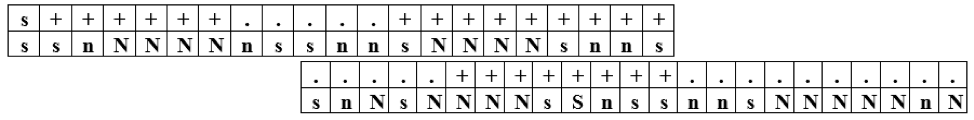
\includegraphics{amelia_fig2.png}
    \caption{\textbf{Output from the program shows results following the expected pattern.}  This example result from the program follows the expected pattern of on and off groups alternating where the on groups roughly follow the areas in which there have been mutations. ‘On’ bits are designated by plusses, ‘off’ groups by periods. Codons with mutations are shown in uppercase, without are shown in lowercase.  The Ns designate codons where the center site is nonsynonymous, the Ss designate codons where the center site is synonymous. This is one of the nicer results from the program, not all follow the pattern.  The program was run with 1000 generations of 100 individuals with a small group cost of -3 and a zero-benefit of 0.5.  All other settings were Pyevolve defaults.}
    \label{fig:my_label}
\end{figure}

\begin{figure}
    \centering
    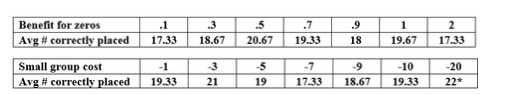
\includegraphics{amelia_fig3.png}
    \caption{\textbf{ Average number of correctly placed bits peaks at small group cost of -3 and zero-benefit of 0.5.}The program was run for 1000 generations of 100 individuals and the average of three samples was taken.  The scores were created by counting the number of ‘on’ bits located with a codon that had a mutation and the number of ‘off’ bits at locations that did not have a mutation.
*In one round, the fitness never got above zero which means the genetic algorithm had nothing to act on.
}
    \label{fig:my_label}
\end{figure}


\section{Acknowledgement}
I would like to thank Dr. Peter Drake for his continued support on this project; Dr. Greta Binford for the skills learned in her phylogenetics class; and Julia Somers for the inspiration for this project.


\bibliographystyle{unsrt}  
%\bibliography{references}  %%% Remove comment to use the external .bib file (using bibtex).
%%% and comment out the ``thebibliography'' section.


%%% Comment out this section when you \bibliography{references} is enabled.
\begin{thebibliography}{1}

\bibitem{aaa}
	Kesh S. and Raghupathi W.  Critical issues in bioinformatics and computing. In “Perspectives in health information management” vol. 1 9. (2004)

\bibitem{bbb}	
Binford G. BIO-408: Phylogenetic Bio & Molec Evol. at Lewis & Clark College. Lecture (2017)
\bibitem{ccc}
Weaver R. F. Molecular Biology. 5th ed., McGraw-Hill. (2012)

\bibitem{ccc}
Nei M. and Gojobori T. Simple Methods for Estimating the Numbers of Synonymous and Nonsynonymous Nucleotide Substitutions. In “Mol. Biol. Evol.” 3(5):418-26 (1986) 

\bibitem{ccc}
Martincorena I, et al. Universal Patterns of Selection in Cancer and Somatic Tissues. In “Cell” 171, 1029–1041 (2017)

\bibitem{ccc}
Eiben A. E. and Smith J. E. Introduction to Evolutionary Computing. Springer, 2003.

\bibitem{ccc}
Cock P. J. A., et al. Biopython: freely available Python tools for computational molecular biology and bioinformatics. In “Bioinformatics” Volume 25, Issue 11, pp 1422–1423 (2009)

\bibitem{ccc}
Perone C. S. Pyevolve. Version 0.5. (2009) http://pyevolve.sourceforge.net/index.html


\end{thebibliography}

\end{document}
